\subsection*{Деревья, наименьший общий предок [14]}
\begin{center}
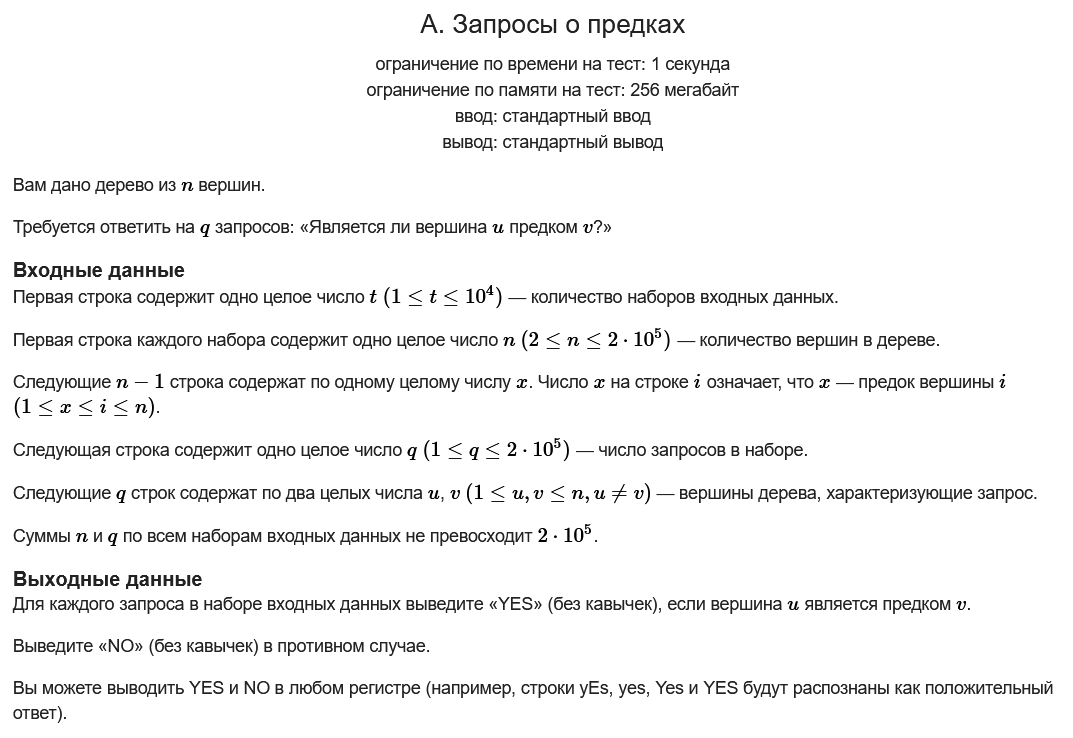
\includegraphics[width=\textwidth]{19A.png}
\end{center}
\subsubsection*{Идея решения}
Введем массивы $tin$ и $tout$ для подсчёта времени входа и выхода соотвественно. Вершина $u$ является предком $v$ тогда и только тогда, когда $tin_v \in [tin_u; tout_u]$. Это условие мы и проверим и выведем ответ. 
\subsubsection*{Исходный код}
\begin{lstlisting}
#include <iostream>
#include <sstream>
#include <fstream>
#include <iomanip>
#include <string>
#include <cstdlib>
#include <cstdio>
#include <cstring>
#include <cmath>
#include <vector>
#include <queue>
#include <algorithm>
using namespace std;
typedef int ll;
const long long size = 10e5 * 2 + 228;
ll n, m;
ll qq = 0;
ll q, v, u;
ll x;
int tin[202222], tout[202222];
vector<vector<ll>> gr;
void dfs(long long v, long long p = -1) {
    tin[v] = qq++;
    for (int i = 0; i < gr[v].size(); i++) {
        dfs(gr[v][i]);
    }
    tout[v] = qq;
    return;
}
int main() {
    ios_base::sync_with_stdio(false);
    cin.tie(0);
    cout.tie(0);
    ll t;
    cin >> t;
    for (int _ = 0; _ < t; _++) {
        cin >> n;
        gr.assign(n,vector<ll>());
       /* tin.assign(n,0), tout.assign(n,0);*/
        for (int i = 1; i <= n - 1; i++) {
            cin >> x;
            gr[x - 1].push_back(i);
        }
        dfs(0);
        cin >> q;
        for (int i = 0; i < q; i++) {
            cin >> u >> v;
            --u, --v;
            if (tin[v] >= tin[u] and tin[v] < tout[u]) {
                cout << "YES";
            }
            else cout << "NO";
            cout << '\n';
        }
      
    }
    return 0;
}
\end{lstlisting}
\subsubsection*{Фрагмент турнирной таблицы контеста}
\begin{center}
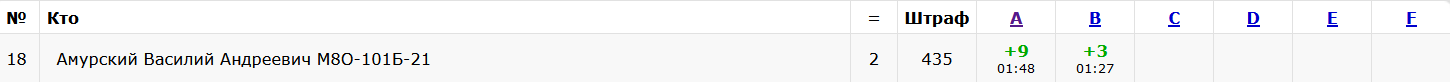
\includegraphics[width=\textwidth]{state19.png}\newline\noindent
\end{center}

\subsubsection*{Выводы}
Задача решена. Основные события процесса отладки: ошибка исполнения на тесте 2, вместо resize использовал assign; превышено ограничение времени на тесте 10, добавил команды cin.tie(0) и сout.tie(0);
